%=======================================================================
%  When Fine-Tuning Beats Fluency
%  An empirical study of small encoder-decoder summarization of product
%  reviews, and of what per-review summaries hide.
%
%  Build:  ./build.sh        (or see README.md)
%  Facts:  EXPERIMENT_FACTS.md is the single source of truth for numbers.
%          Never quote a number that is not in that file.
%=======================================================================

\documentclass[conference]{IEEEtran}

\usepackage{cite}
\usepackage{amsmath,amssymb}
\usepackage{graphicx}
\usepackage{booktabs}
\usepackage{url}
\usepackage[hidelinks]{hyperref}

% Nicer tables: no vertical rules, a little breathing room.
\renewcommand{\arraystretch}{1.15}

\begin{document}

\title{When Fine-Tuning Beats Fluency:\\
Small Encoder--Decoder Summarization of Product Reviews\\
and What Per-Review Summaries Hide}

\author{
\IEEEauthorblockN{Raviraj Ladha}
\IEEEauthorblockA{M.Tech.\ Artificial Intelligence and Machine Learning\\
BITS Pilani, Work Integrated Learning Programmes\\
ravirajladha@gmail.com}
}

\maketitle

\begin{abstract}
% STATUS: draft written, session 1. Revisit last, once results are final.
% LENGTH: 150-200 words.
Automatic summarization of product reviews is usually framed as a modelling
problem, but on real e-commerce data it is equally a problem of \emph{form}.
We fine-tune \texttt{t5-small}, a 60M-parameter encoder--decoder, on 4{,}000
Amazon food reviews whose reference summaries are the headlines customers
wrote themselves, and evaluate on 300 held-out reviews. Fine-tuning improves
ROUGE-1 from 0.109 to 0.175, a relative gain of 61\%. The more instructive
result is the baseline: the \emph{same pretrained model without fine-tuning}
scores 0.109, below the 0.126 of a trivial extractive baseline that simply
returns the first sentence. The un-tuned model is fluent and on-topic, but
writes full sentences where the task rewards a four-word headline; fluency is
not task fit. We further show that per-review summarization, while accurate,
systematically conceals aggregate signal: for a baby-formula product with a
3.13 star average and predominantly positive summaries, aspect mining over the
same reviews surfaces sustained complaints about arsenic levels and infant
health. We argue that review summarization systems should be evaluated at the
aggregate level, not only per review.

\end{abstract}

\begin{IEEEkeywords}
abstractive summarization, encoder--decoder, transfer learning, opinion
mining, aspect extraction, ROUGE, low-resource evaluation
\end{IEEEkeywords}

\section{Introduction}
% STATUS: stub. SESSION 3.
% GOAL: ~1 page. Motivate, state contributions, forward-reference results.
% MUST CONTAIN:
%   - The buyer problem: thousands of reviews, nobody reads them all.
%   - Framing: two sub-problems, per-review compression AND aggregation.
%   - The surprise: pretrained-but-untuned < trivial baseline. Say the number.
%   - Contributions list (3 items, matching EXPERIMENT_FACTS.md "can claim").
%   - Honesty: single dataset, single seed, small model. Say it here, not only
%     in Limitations.
% CITE: \cite{raffel2020t5} for the model, \cite{mcauley2013amazon} for data.

TODO

\section{Related Work}
\label{sec:related}

\textbf{Encoder--decoder summarization.} Abstractive summarization inherits its
architecture from neural machine translation. Sutskever et al.
\cite{sutskever2014seq2seq} showed that a recurrent encoder could compress a
variable-length input into a fixed-length vector from which a decoder generates
the output. That fixed-length vector is also the approach's weakness: a single
state must carry an entire document, and the longer the document the more it
must discard. Bahdanau et al. \cite{bahdanau2015attention} removed the
bottleneck by letting the decoder attend over all encoder states, learning a
soft alignment between output and input positions. Vaswani et al.
\cite{vaswani2017attention} then discarded recurrence entirely in favour of
self-attention. Within summarization specifically, See et al.
\cite{see2017pointer} addressed two failure modes of the recurrent formulation
--- inability to reproduce rare words, and repetition --- with a pointer
mechanism that copies from the source and a coverage penalty. Our recurrent
baseline follows this lineage, using additive attention
\cite{bahdanau2015attention}, though we did not train it (Section~\ref{sec:limitations}).

\textbf{Pretraining and its benchmarks.} Pretraining changed the cost structure
of the task: a general model is adapted with comparatively little in-domain
data. T5 \cite{raffel2020t5} casts every task as text-to-text and selects among
them with a textual prefix, which is the model and the mechanism we use. Liu
and Lapata \cite{liu2019bertsum} adapted a pretrained encoder to both
extractive and abstractive summarization, and PEGASUS \cite{zhang2020pegasus}
introduced a pretraining objective designed for summarization specifically.

These systems are, with few exceptions, developed and reported on news
corpora, where a reference summary is a paragraph or --- in the most compressed
case --- a single sentence. Our references are neither. They are headlines a
customer typed into a form, averaging four words. This is not a minor
difference of degree: it changes what the standard metric can measure, which we
take up in Section~\ref{sec:analysis}. We stress it here because it is the main
reason absolute ROUGE values in this paper should not be read against the
numbers those systems report.

\textbf{Opinion summarization.} Summarizing many reviews of one product is a
distinct problem, and it is usually attacked without reference summaries, since
no customer writes a summary of everyone else's opinions. MeanSum
\cite{chu2019meansum} trains an unsupervised model to generate a single review-
like summary whose encoding stays close to the mean of the input reviews.
Bra\v{z}inskas et al. \cite{brazinskas2020fewshot} showed that a small number of
annotated summaries is enough to adapt such a model. Both produce one fluent
paragraph per product. We differ in output rather than ambition: we combine
per-review summaries through a map--reduce procedure and pair them with a
structured list of praised and criticised aspects, because a fluent paragraph
is precisely the format in which a minority complaint disappears --- the effect
we document in Section~\ref{sec:analysis}.

\textbf{Evaluation.} ROUGE \cite{lin2004rouge} remains the default and was
designed against multi-sentence references. Its limits are well documented:
BERTScore \cite{zhang2020bertscore} replaces surface overlap with contextual
embedding similarity, and SummEval \cite{fabbri2021summeval} found that
automatic metrics, ROUGE included, correlate weakly with human judgement.
Maynez et al. \cite{maynez2020faithfulness} showed further that overlap metrics
are largely blind to faithfulness, since a summary can score well while
asserting something the source does not support. We report ROUGE, and
Section~\ref{sec:analysis} sets out what we believe it does and does not
establish in our setting.

\section{Data}
% STATUS: stub. SESSION 2 -- do this first, it is the most mechanical.
% GOAL: ~0.5 page + one table. All numbers from EXPERIMENT_FACTS.md sec.2.
% MUST MAKE THE CENTRAL POINT: mean summary length is 4.1 words. The reference
%   is a headline, not an abstract. Every later argument leans on this.
% ALSO: 78.1 percent of reviews are 4-5 star (label skew); filter keeps 84.6
%   percent; splits 4000/300/500 with 300 actually scored; seed 42.
% CITE: \cite{mcauley2013amazon}.

TODO

\section{Method}
\label{sec:method}

The system has three parts: a per-review summarizer, a map--reduce procedure
that extends it to many reviews, and an aspect miner that answers the question
the summarizer structurally cannot.

\subsection{Per-review summarization}

We fine-tune \texttt{t5-small} \cite{raffel2020t5} on (review, headline) pairs.
T5 is a multi-task text-to-text model in which the task is selected by a
textual prefix, so each input is prepended with \texttt{"summarize: "}.
Decoding uses beam search with four beams and blocks repeated bigrams; without
the latter the model degenerates into repetition (\emph{``good good good''}) on
targets this short.

\subsection{Map--reduce aggregation}

A product page carries tens or hundreds of reviews, and the encoder accepts at
most 256 tokens. Concatenating the reviews and passing them in one call does
not fail --- it silently truncates, so most reviews never influence the output
at all. We therefore aggregate in two stages, following the map--reduce shape:
each review is summarised independently (\emph{map}), the resulting summaries
are joined into a single pseudo-document, and that document is passed back
through the same model (\emph{reduce}) with a doubled generation budget.

This raises the ceiling but does not remove it, and we state the consequence
plainly: the reduce step is itself subject to the 256-token encoder limit. With
per-review summaries averaging four to six tokens, a single reduce pass
saturates somewhere around forty to fifty reviews, beyond which the later
summaries are truncated exactly as the raw reviews would have been. A
hierarchical reduce --- reducing in batches, then reducing the results ---
would remove the ceiling entirely. We did not implement it, and the
demonstration in Section~\ref{sec:analysis} uses sixty reviews, which is inside
the regime where mild truncation is possible. This is a limitation of our
implementation, not of the approach.

\subsection{Aspect mining}

Neither a per-review summary nor a reduced summary answers the question the
task actually poses --- which aspects do customers as a group praise, and which
do they criticise. That answer is a property of the collection, not of any
review in it. We compute it separately.

Reviews are split into sentences and each sentence is scored with VADER
\cite{hutto2014vader}, a rule-based sentiment analyser. Sentences above $+0.2$
form the positive pool and those below $-0.2$ the negative pool; the stricter
sentence threshold means only clearly polar sentences contribute aspects. A
separate, looser threshold of $\pm0.05$ on the whole review is used for the
positive/negative/neutral counts reported to the user.

Candidate aspects are unigrams and bigrams, with English stop words removed
along with a hand-built list of \emph{opinion} words. This second list matters:
terms such as \emph{good}, \emph{love} and \emph{disappointed} carry the
verdict rather than the topic, and terms such as \emph{product},
\emph{amazon} and \emph{bought} are true of every review. Neither identifies
what is being discussed.

Ranking candidates by raw frequency does not work. For a cat toy, \emph{cat}
and \emph{toy} head both lists, and praise and criticism look identical. We
instead select \emph{contrastively}: a term is listed on a side only if the
share of its usage falling on that side, measured as a rate rather than a raw
count because the two pools differ in size, is at least $0.6$ --- that is,
mentioned at least $1.5\times$ more often there. Terms with fewer than two
mentions are dropped as noise. Finally, a unigram is discarded when it is
dominated by a bigram containing it, so \emph{battery life} is preferred to
\emph{battery} while a standalone \emph{flavor} survives.

We emphasise what this is not. It is a frequency-and-polarity heuristic, not a
trained aspect-based sentiment model. It identifies \emph{what} is discussed on
each side; it cannot resolve a negated aspect inside an otherwise positive
sentence.

\subsection{The reported verdict}

The paragraph the application shows is assembled from three sources rather
than generated end to end, and we describe it as such. A mood phrase is chosen
from the share of \emph{polar} reviews that are positive --- neutral reviews
are excluded from this ratio deliberately, since counting them drags a
genuinely mixed product toward ``unhappy'' --- followed by the top five
praised and criticised aspects, followed by the reduce step's generated
sentence quoted verbatim. The neural component contributes the summaries and
the quoted verdict; the structure around it is a template.

\section{Experimental Setup}
% STATUS: stub. SESSION 2 (pairs naturally with Data).
% GOAL: ~0.5 page. Everything needed to reproduce.
% Hyperparameters table from EXPERIMENT_FACTS.md sec.3.
% Baselines and why each: Lead-1 (is the task trivially extractive?),
%   un-tuned t5-small (does fine-tuning do anything at all?).
% Hardware: CPU only, ~112 min. NOTE: README says ~50 min for the same run.
%   RESOLVE THIS before writing. Do not cite a number you have not checked.
% Metric: ROUGE-1/2/L \cite{lin2004rouge}, HuggingFace evaluate.

TODO

\section{Results}
\label{sec:results}

Table~\ref{tab:rouge} and Figure~\ref{fig:rouge} report ROUGE against the
customer-written headline on the 300 held-out reviews. We state the outcomes
here and defer their interpretation to Section~\ref{sec:analysis}.

\begin{table}[t]
\caption{ROUGE on 300 held-out reviews. Best in bold.}
\label{tab:rouge}
\centering
\begin{tabular}{lccc}
\toprule
\textbf{Model} & \textbf{ROUGE-1} & \textbf{ROUGE-2} & \textbf{ROUGE-L} \\
\midrule
Lead-1 (extractive)        & 0.1255 & 0.0341 & 0.1145 \\
\texttt{t5-small}, not tuned & 0.1086 & 0.0266 & 0.0974 \\
\texttt{t5-small}, fine-tuned & \textbf{0.1751} & \textbf{0.0448} & \textbf{0.1723} \\
\bottomrule
\end{tabular}
\end{table}

\begin{figure}[t]
\centering
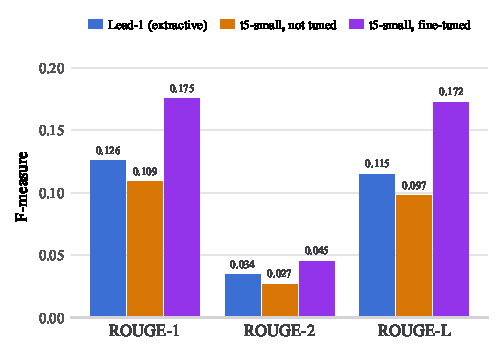
\includegraphics[width=\columnwidth]{figures/rouge_comparison.pdf}
\caption{ROUGE by model. The un-tuned pretrained model (centre) falls below the
extractive Lead-1 baseline (left) on all three measures.}
\label{fig:rouge}
\end{figure}

Three observations follow directly from the table.

\textbf{Fine-tuning helps substantially.} The fine-tuned model improves
ROUGE-1 from 0.1086 to 0.1751 over the same checkpoint untuned, a relative gain
of 61.2\%, with consistent gains on ROUGE-2 (+68.4\%) and ROUGE-L (+76.9\%).

\textbf{The task is not trivially extractive.} The fine-tuned model also beats
Lead-1, 0.1751 against 0.1255, a relative gain of 39.5\%. Lead-1 is a stronger
baseline than it may appear: customers frequently reuse their opening words in
their headline, so returning the first sentence captures real signal.

\textbf{The un-tuned pretrained model loses to Lead-1.} At 0.1086 against
0.1255 it scores 13.5\% below a baseline that performs no modelling at all, and
it does so on all three measures rather than on one. This is the result we
consider most informative, and Section~\ref{sec:analysis} takes it up.

Two properties of these numbers should be read carefully. First, all values are
low in absolute terms, and ROUGE-2 in particular sits near its floor; this is a
consequence of the reference length established in Section~\ref{sec:data} and
not, we argue, of the systems being uniformly poor. Second, \textbf{we ran no
significance test}, so we make no claim about whether any individual difference
would survive one. The 61.2\% and 13.5\% gaps are large relative to the values
involved, and the ordering is consistent across all three measures, but
consistency across correlated metrics is weak evidence and we do not present it
as more.

\subsection{Qualitative behaviour}

Table~\ref{tab:examples} pairs generated summaries with the customer headline
for four held-out reviews. The model produces short, headline-shaped output of
the register the task calls for. The final row is the informative failure: the
review praises a dog treat and then complains at length about the flatulence it
caused, and the model retains the praise while discarding the complaint.

\begin{table}[t]
\caption{Generated summaries against the customer's own headline.}
\label{tab:examples}
\centering
\begin{tabular}{p{0.44\columnwidth}p{0.42\columnwidth}}
\toprule
\textbf{Customer headline} & \textbf{Generated} \\
\midrule
totally worth the money!!! & he loves it! \\
i like this stuff!         & i love this cereal! \\
best i have found          & good taste, good quality \\
offensive gas producer!!!  & a great treat! \\
\bottomrule
\end{tabular}
\end{table}

\section{Analysis}
% STATUS: stub. SESSION 7. This is the paper's real contribution -- give it
%   the most care and the most space (~1.25 pages).
% 7.1 Why fluency loses. Un-tuned model writes grammatical sentences; the
%     reference is a 4-word headline. Right content, wrong shape. Use the
%     qualitative pairs in EXPERIMENT_FACTS.md sec.5.
% 7.2 What ROUGE can and cannot say here. With ~4-word references there are
%     very few bigrams, so ROUGE-2 sits near its floor. Absolute values are
%     NOT comparable to news benchmarks \cite{zhang2020pegasus}. Argue the
%     comparison between systems is still valid; the absolute number is not.
%     Concede \cite{fabbri2021summeval}, \cite{zhang2020bertscore}.
% 7.3 The aggregation finding. Baby formula, 3.13 stars, positive summaries,
%     yet criticism list = arsenic / health / constipation. Quote the generated
%     summaries in EXPERIMENT_FACTS.md sec.6. THIS IS THE STRONGEST RESULT.
% 7.4 Error analysis. "offensive gas producer!!!" -> "a great treat!": the
%     model keeps praise and drops the complaint. Connect to
%     \cite{maynez2020faithfulness}. Mixed-polarity reviews are the weak spot,
%     and they are exactly the informative ones.

TODO

\section{Limitations}
% STATUS: stub. SESSION 8. Be ruthless here -- it is what makes the rest
%   credible. Everything in EXPERIMENT_FACTS.md "cannot claim" goes in.
% - No from-scratch baseline: the LSTM is implemented but never trained.
% - One dataset, one domain, one model size, one seed, one epoch.
% - No significance testing.
% - Eval-set-size observation (24 -> 0.234 vs 300 -> 0.174) is anecdotal.
% - Aspect miner: frequency-based, no negation handling, singular/plural not
%   collapsed across lists (formula praised while formulas criticised).
% - No human evaluation, no faithfulness metric.

TODO

\section{Conclusion}
% STATUS: stub. SESSION 8.
% GOAL: ~0.3 page. Two claims, one recommendation. No new information.
%   1. Task fit, not fluency, is what fine-tuning buys on headline-style refs.
%   2. Per-review summarization conceals aggregate signal that matters.
%   -> Recommendation: evaluate review summarizers at the aggregate level.

TODO


% TEMPORARY: while the sections are still stubs, no \cite command is actually
% live, so the bibliography would print empty. \nocite{*} forces every entry in
% references.bib to appear, which doubles as a reading list.
% DELETE THIS LINE once the sections cite properly (around session 6).
\nocite{*}

\bibliographystyle{IEEEtran}
\bibliography{references}

\end{document}
